\documentclass[technical_document.tex]{subfiles}
\begin{document}
\section{Software design}
Eva\textquotesingle s software \footnote{http://code.google.com/p/roman-technologies} is implemented in C++, using ROS 
\footnote{http://www.ros.org/wiki/} . In the implemented software structure, each package represents a physical part of Eva, with a 
logical\_unit package acting as her ``brain'', which receives data from Eva\textquotesingle s sensors and encoders and which makes decisions based on the readings. The decisions made by the logical\_unit result in actions that have to be executed 
by the physical parts of Eva, in other words, the logical unit will generate commands for the other packages to execute. 
Figure \ref{fig:implementation} shows the structure of the software packages. External packages implemented by third 
parties are shown in the notes in the figure. Also, feedback from the slaves to the main Controller are not shown to keep 
the image clear.

The structure can also be seen as a modification of the master-slave model, \footnote{http://en.wikipedia.org/wiki/Master-slave\_(technology)} with extra submasters and feedback providing slaves. 
Looking inside the packages, a ``main'' master can be identified (Controller in logical\_unit), 
there are submasters (The ``AutonomeController'' nodes in the other packages) and there are slaves which provide 
feedback to the ``main'' master (all the other nodes). This way, the main master in the logical\_unit can adjust to the 
data provided by the slaves, resulting in better control of the whole system. By having submasters in the structure, the 
responsibility of the main master is reduced and distributed over the submasters. 

In software engineering, designs should be loosely coupled, yet highly cohesive \footnote{http://www.xyzws.com/scjp/SGS11/5/2} . In this design, loose coupling was automatically achieved because of the 
ROS framework. In ROS, nodes communicate with each other through topics or services. A node can call a service on 
another node, or it can post its data on a topic which is accesible for any node in ROS. Especially when topics are used, 
these nodes can run completely independent from the other nodes, making the entire system loosely coupled. One could 
remove a node in the ROS system without destroying other nodes and replace it with another one. As long as this new node 
keeps the protocol between the old node and the rest of the system intact (meaning that it listens and broadcasts to the 
same topics or services), this node may have an entirely different implementation.

High cohesion is achieved by splitting the software in packages, each package is then assigned a specific task. As mentioned before, each package represents a physical ``body'' part of Eva, such as her arm, mobile base, sensors etc. This way, each package is specialized in one part of the robot and only contains nodes to provide functionality within that package and one node to communicate with the rest of the system (the AutonomeController node in that package and teh Controller node in logical\_unit). Also, the input for Eva is split apart in two different packages: image\_processing and audio\_processing, increasing the cohesion of the entire system. 


\begin{figure}[ht!]
	\centering
	\mbox{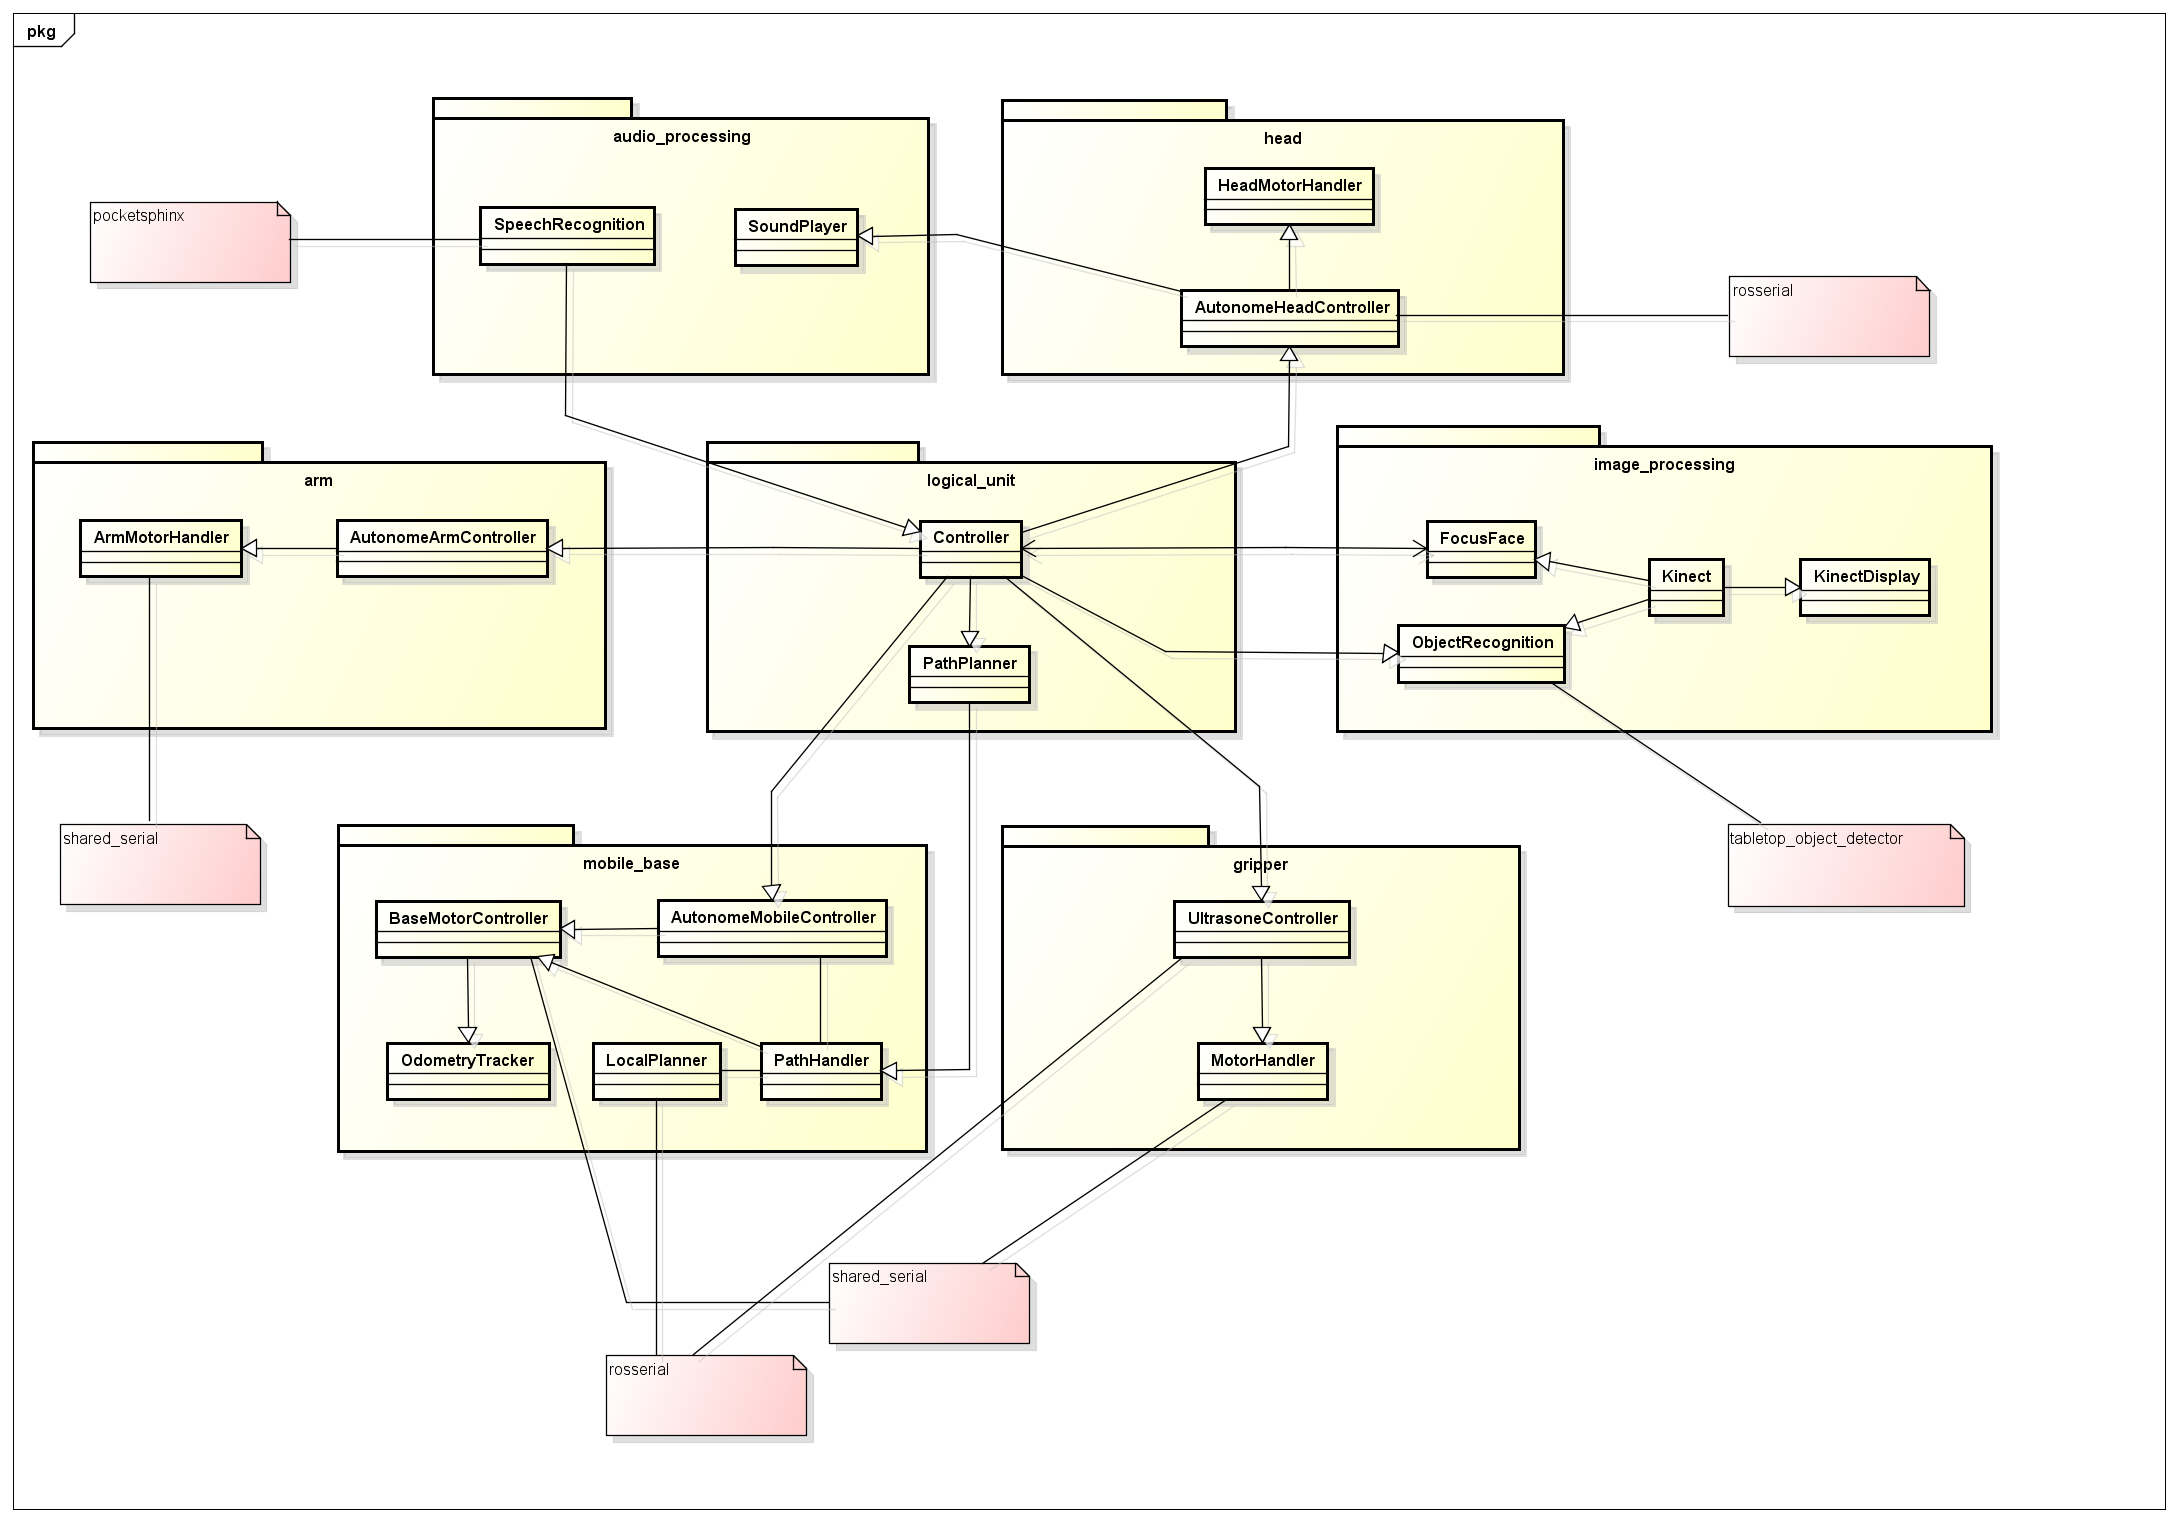
\includegraphics[scale=0.3]{Images/nodes.png}}
	\caption{Structure of the packages as in the implementation and the nodes within it.}
	\label{fig:implementation}
\end{figure}

\end{document}
